\documentclass[12pt]{article}
\usepackage{amsmath}
\usepackage{amssymb}
\usepackage{amsfonts}
\usepackage{polski}
\usepackage[utf8]{inputenc}
\usepackage[OT4]{fontenc}
\usepackage{graphicx}
\usepackage{float}




\textheight 23.2 cm

\textwidth 6.0 in

\hoffset = -0.5 in

\voffset = -2.4 cm

\hyphenation{me-to-dy la-bo-ra-to-rium}

\begin{document}

%h�?
%\thispagestyle{empty}

\vspace*{3ex}
\begin{flushright}
{\large 11 stycznia 2022 r.}
\end{flushright}

\begin{flushleft}
{\large Mateusz Andryszak\\
322422}
\end{flushleft}

\hskip3cm

\begin{center}

\Large {\bf Metoda Gaussa-Seidela dla równań macierzowych $AX = B$ oraz $XA = B$ }

\vskip2ex

{\large Projekt nr 2}

\end{center}

\vskip20ex



\section{Opis metody}

\noindent Za zadanie mamy wyznaczyć macierz $X$ spełniającą jedno z poniższych równań:
\begin{equation} \label{eq:eq1}
    AX=B
\end{equation}
gdzie $A \in \mathbb{R}^{n \times n}, \hskip2ex B\in \mathbb{R}^{n \times m}$ 

\begin{equation} \label{eq:eq2}
    XA=B
\end{equation}
gdzie $A \in \mathbb{R}^{n \times n}, \hskip2ex B\in \mathbb{R}^{m \times n}$\\


za pomocą metody iteracyjnej Gaussa-Seidela.\\

\noindent Do wyznaczenia macierzy $X$ posłużymy się macierzą iteracyjną.
\\
Przedstawiamy macierz $A$ jako sumę trzech macierzy $A=L+D+U$, gdzie \\
L jest macierzą trójkątną dolną zawierającą elementy leżące pod
diagonalą $A$, $D$ jest macierzą diagonalną, zawierająca elementy diagonali $A$, a $U$ jest macierzą trójkątną górną zawierającą elementy leżące ponad diagonalą $A$ \\

Dla równania (\ref{eq:eq1}):\\

\[
AX=(L+D+U)X=(L+D)X+UX=B
\]
\[
(L+D)X=-UX+B
\]
\[
X=-(L+D)^{-1}UX+(L+D)^{-1}B
\]
Dla odpowiedniej iteracji:
\[
X^{(k+1)}=-(L+D)^{-1}UX^{(k)}+(L+D)^{-1}B,\hskip2ex k=0,1,...
\]
Czyli oznaczając odpowiednie macierze:
\[
X^{(k+1)}=B_{gs}X^{(k)}+C_{gs},\hskip2ex k=0,1,...
\]
gdzie:
\[
B_{gs}=-(L+D)^{-1}U, a C_{gs}=(L+D)^{-1}B
\]\\


Dla równania (\ref{eq:eq2}):\\

\[
XA=X(L+D+U)=X(L+D)+XU=B
\]
\[
X(L+D)=-XU+B
\]
\[
X=-XU(L+D)^{-1}+B(L+D)^{-1}
\]
Dla odpowiedniej iteracji:
\[
X^{(k+1)}=-X^{k}U(L+D)^{-1}+B(L+D)^{-1},\hskip2ex k=0,1,...
\]
Czyli oznaczając odpowiednie macierze:
\[
X^{(k+1)}=B_{gs}X^{(k)}+C_{gs},\hskip2ex k=0,1,...
\]
gdzie:
\[
B_{gs}=-U(L+D)^{-1}, a C_{gs}=B(L+D)^{-1}
\]


\section{Opis programu obliczeniowego}

\noindent Funkcja $gaus\_seidel$ służy do wyznaczenia macierzy $X$ z równania $AX=B$\\
Funkcja $gaus\_seidel\_2$ służy do wyznaczenia macierzy $X$ z równania $XA=B$\\ \\
Obie funkcje przyjmują 5 parametrów:\\

$A$ - Macierz $A$ z równania\\

$B$ - Macierz $B$ z równania\\

$max\_iterations$ - parametr opcjonalny określający maksymalną ilość iteracji. W przypadku braku parametru $max\_iterations$ przy wywołaniu funkcji jest on ustawiony na $max\_iterations=100$\\

$tolerance$ - parametr opcjonalny określający dokładność wyniku, przy której kolejna iteracja nie zostanie już wykonana. W przypadku braku parametru $tolerance$ przy wywołaniu funkcji jest on ustawiony na $tolerance=0.00001$\\

$A_0$ - parametr opcjonalny określający przybliżenie początkowe macierzy $X$. W przypadku braku parametru $A_0$ przy wywołaniu funkcji jest on ustawiony na $X=\mathbf{0}$\\\\

\noindent Funkcja $gaus\_seidel$ zwraca trzy wartości:\\

$X$ - szukana macierz $X$\\

$error$ - błąd szukanej macierzy\\

$r$ - promień spektralny macierzy $B_{gs}$\\

\noindent Błąd obliczamy za pomocą normy: $error=norm(GoodX-X)$ gdzie
$GoodX$ jest macierzą obliczoną za pomocą operacji na macierzach. Zakładamy, że macierz $A$ jest odwracalna. W przypadku gda macierz $A$ nie jest odwracalna, program zadziała, lecz błąd nie zostanie policzony.


\section{Przykłady obliczeniowe}
\noindent Program został przetestowany na wielu przykładach.

\begin{enumerate}
    \item \textbf{Rozwiązywanie układu równań liniowych - promień spektralny macierzy $B_{gs}$ mniejszy od 1}\\
    Jako przykład bierzemy macierze:
    \[
    A=\begin{pmatrix}
2 & 1 \\
1 & 2 \\
\end{pmatrix},\hskip3ex
    B=\begin{pmatrix}
8 \\
1 \\
\end{pmatrix}
    \]
    parametrów opcjonalnych nie dodajemy. \\
    Po zastosowaniu funkcji $gaus\_seidel$ macierz $B_{gs}=\begin{pmatrix}
0 & -0.5 \\
0 & 0.25 \\
\end{pmatrix}$

więc jej promień spektralny jest mniejszy od 1, a gdy promień spektralny macierzy iteracyjnej jest mniejszy od 1 to metoda gaussa-seidela jest zbieżna globalnie. Dla wystarczającej ilości iteracji, otrzymany błąd dla danego przykładu jest bliski 0.
    

    \item \textbf{Rozwiązywanie układu równań liniowych - promień spektralny macierzy $B_{gs}$ większy od 1}\\
    Jako przykład bierzemy macierze:
    \[
    A=\begin{pmatrix}
1 & 1 & 1\\
1 & 2 & 2\\
1 & 3 & 1\\
\end{pmatrix},\hskip3ex
    B=\begin{pmatrix}
7 \\
13 \\
13\\
\end{pmatrix}
    \]
    parametrów opcjonalnych nie dodajemy. \\
Po zastosowaniu funkcji $gaus\_seidel$ macierz $B_{gs}=\begin{pmatrix}
0 & -1 & -1 \\
0 & 0.5 & -0.5 \\
0 & -0.5 & 2.5 \\
\end{pmatrix}$

więc jej promień spektralny jest większy od 1, a gdy promień spektralny macierzy iteracyjnej jest większy od 1 to metoda gaussa-seidela nie jest zbieżna globalnie, a w naszym przypadku dla początkowego przybliżenia macierzy $X=\mathbf{0}$ metoda jest rozbieżna i błąd jest duży. Jednak w podanym przykładzie wystarczy zamiana wierszy drugiego z trzecim w macierzach $A$ i $B$ aby metoda zadziałała w celu znalezienia rozwiązań układu równań.
    
    \item \textbf{Macierz przekątniowo dominująca}\\
    Stwórzmy dowolną macierz $A$ taką, żeby na pewno byla przekątniowo dominująca:\\
    $A=(rand(4)+3*eye(4))*100$\\
    Następnie weźmy dowolną macierz $B$:\\
    $B_1=rand(4,3)$, \hskip3ex
    $B_2=rand(5,4)$\\

    Dla każdych takich macierzy funkcje $gaus\_seidel(A,B_1)$ oraz $gaus\_seidel\_2(A,B_2)$ są zbieżne globalnie, gdyż jeżeli macierz $A$ jest przekątniowo dominująca to macierz iteracyjna ma promień spektralny mniejszy od 1. Dla wystarczającej ilości iteracji, błąd w takich przykładach będzie bliski zera.
    
    \item \textbf{Promień spektralny macierzy $B_{gs}$ jest większy od jeden, jednak wynik jest poprawny} \\
    Jako przykład bierzemy macierze:
    \[
    A=\begin{pmatrix}
1 & 20 & 32 \\
10 & 3 & 18 \\
10 & 20 & 6 \\
\end{pmatrix},\hskip3ex
    B=\begin{pmatrix}
0 & 0 & 0 \\
0 & 0 & 0 \\
0 & 0 & 0 \\
\end{pmatrix}
    \]
    parametrów opcjonalnych nie dodajemy. \\
    
    Po zastosowaniu dowolnej z funkcji $gaus\_seidel$, $gaus\_seidel\_2$, mimo tego, że promień spektralny macierzy $B_{gs}$ jest znacznie większy od 1 to wynik jest poprawny, ponieważ początkowe przybliżenie jest od razu przybliżeniem dobrym.

    \item \textbf{AX=XA=B}\\
    Jako przykład bierzemy macierze:
    \[
    A_1=rand(3),\hskip3ex
    B=\begin{pmatrix}
1 & 0 & 0 \\
0 & 1 & 0 \\
0 & 0 & 1 \\
\end{pmatrix}
    \]

    Okazuje się, że wynik funkcji $gaus\_seidel$ będzie taki sa jak wynik funkcji $gaus\_seidel\_2$, jeżeli użyjemy tą samą liczbę iteracji oraz tą samą macierz początkową. Nie ma znaczenia czy metoda jest zbieżna czy nie. Dzieje się tak, ponieważ:
    \[
    X=-(L+D)^{-1}UX+(L+D)^{-1}B \iff AX=B
    \]
\[
X=-XU(L+D)^{-1}+B(L+D)^{-1} \iff XA=B
\]
\[
AX=XA \iff -XU(L+D)^{-1}+B(L+D)^{-1}=-(L+D)^{-1}UX+(L+D)^{-1}B
\]
    więc każda kolejna iteracja, będzie zwracała ten sam wynik.

    \item \textbf{Za mała ilość iteracji}\\
    Jako przykład bierzemy macierze:
    \[
    A=\begin{pmatrix}
4 & 1 & 2 \\
3 & 5 & 1 \\
1 & 1 & 3 \\
\end{pmatrix},\hskip3ex
    B=\begin{pmatrix}
4 \\
7 \\
3 \\
\end{pmatrix}
    \]
Po zastosowaniu funkcji $gaus\_seidel(A,B,2)$ otrzymamy błąd $e1\approx0.1$\\
Po zastosowaniu funkcji $gaus\_seidel(A,B,3)$ otrzymamy błąd $e1\approx0.02$\\
Po zastosowaniu funkcji $gaus\_seidel(A,B)$ otrzymamy błąd bardzo bliski 0\\

Jeżeli przykład jest zbieżny, wraz ze wzrostem iteracji wzrasta dokładność  wyniku i tym samym maleje błąd.
\end{enumerate}

\section{Analiza wyników}

Metoda działa zawsze jeżeli promień spektralny macierzy $B_{gs}$ jest mniejszy od 1. Dzieję się tak zawsze gdy macierz $A$ jest przekątniowo dominująca i jest to warunek wystarczający zbieżności globalnej. Macierz B może być dowolna, gdyż od niej nie zależy to czy metoda będzie zbieżna. Natomiast w przypadku gdy macierz  $B_{gs}$ ma promień spektralny większy od 1, metoda może zadziałać jeżeli iteracja trafi akurat na wartość bliską poprawnego wyniku. Jednak wydarzy się to tylko dla nielicznie wybranych przybliżeń początkowych, a dla większości metoda będzie rozbieżna. Dodatkowo możemy zauważyć, że wraz ze wzrostem promienia spektralnego macierzy $B_{gs}$ rośnie błąd wyniku. Obrazuje to poniższy wykres stworzony na podstawie wylosowanych macierzy.

\begin{figure}[H]
    \centering
    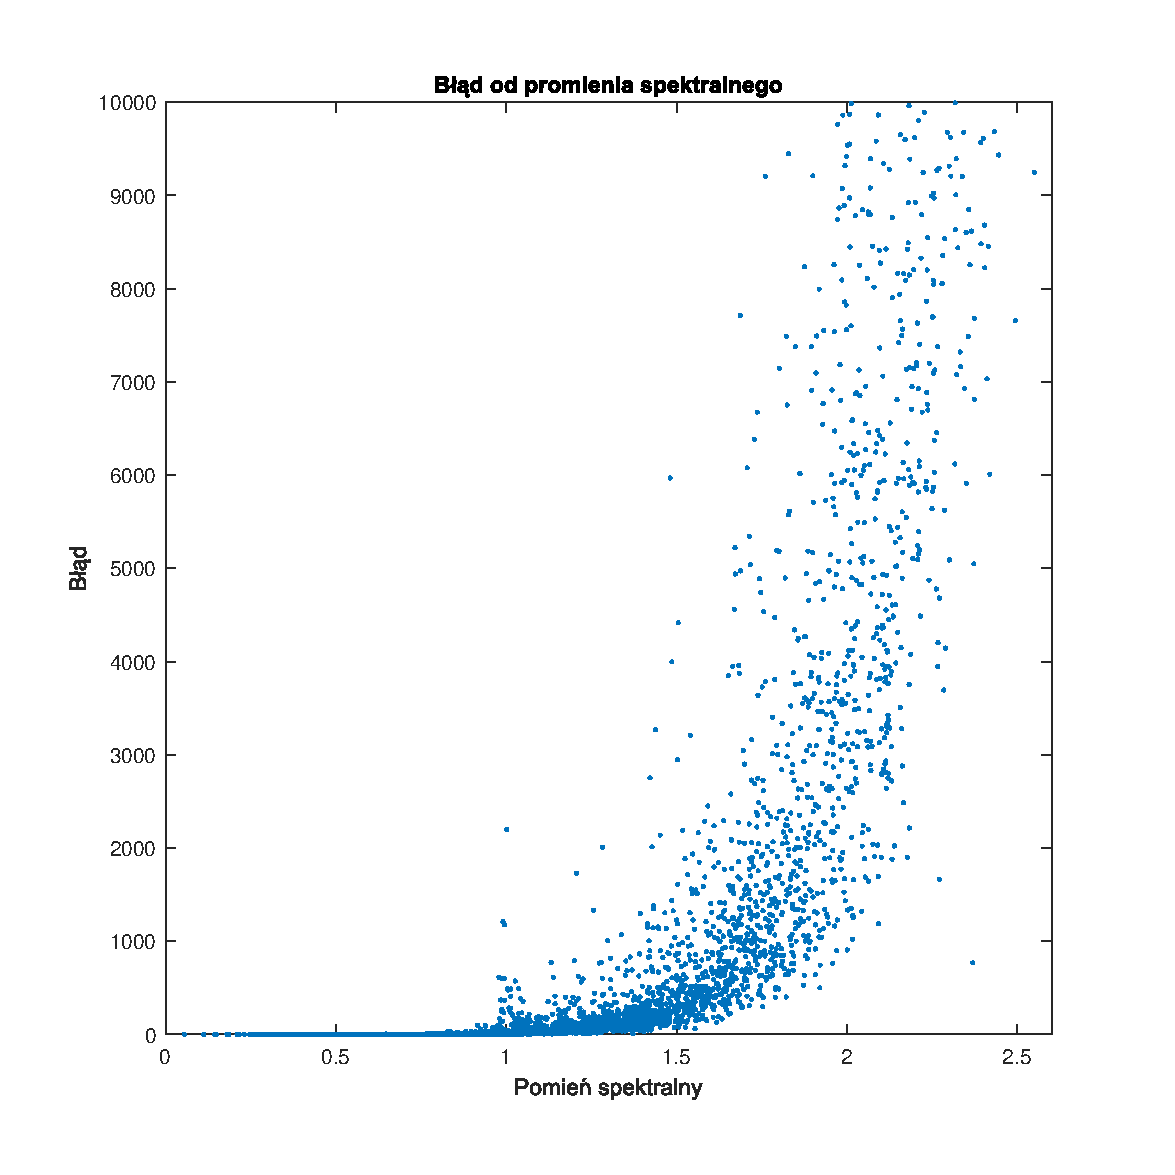
\includegraphics[width=450pt]{graph1.eps}

    \label{label}
\end{figure}

\end{document}
